\section{Duplex: Devices for Efficient LLM Inference}
\label{sec:duplex}
To address the challenges in the hetero system, we propose \duplex, which configures separate processing units for high-\opb and low-\opb operations that share device memories.
Appropriate processing units are selected for each operation based on the stage.
The low-\opb unit handles the MoE layers during the \deconlystage as well as the attention layers of the \deconlystage and of decoding sequences in the \mixedstage.
The high-\opb unit manages the rest.
We opt for an HBM-based system to provide high memory bandwidth.



\subsection{Implementation of High Op/B Processors}
\label{sec:duplex_implement_high_opb}

For high-\opb operations, conventional accelerators, such as GPUs and TPUs, are eligible candidates for a high \opb processor. 
We assume that a popular GPU architecture equipped with HBM serves as a high \opb processor for \duplex.
Hereafter, we refer to the processor as \highp.
Numerous processing units in \highp provide extremely high computational throughput, but the HBM bandwidth is limited due to the physical limitations of the interposer connecting HBM stacks with the main computing die.




\subsection{Implementation of Low Op/B Processors}

\label{sec:duplex_implement_low_opb}


\begin{figure}[!tb]
  \center
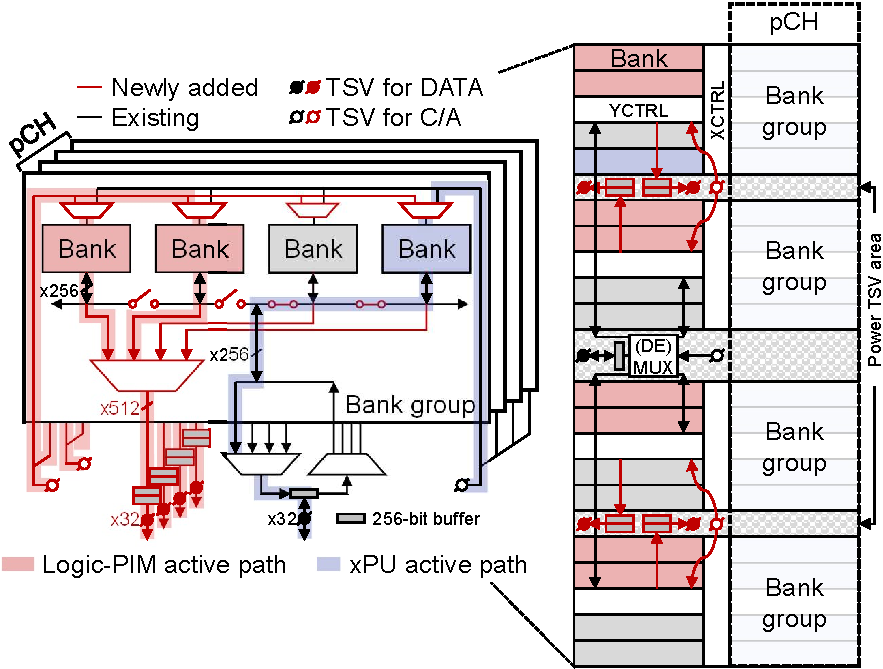
\includegraphics[width=1.0\columnwidth]{figures/microarchitecture.pdf}
  \vspace{-0.1in}
  \caption{Our DRAM die microarchitecture of HBM3 for \lowp. \lowp and xPU can operate simultaneously through independent active paths.}
  \label{fig:duplex_microarchitecture}
  \vspace{-0.1in}
\end{figure}

\begin{figure*}[!tb]
  \center
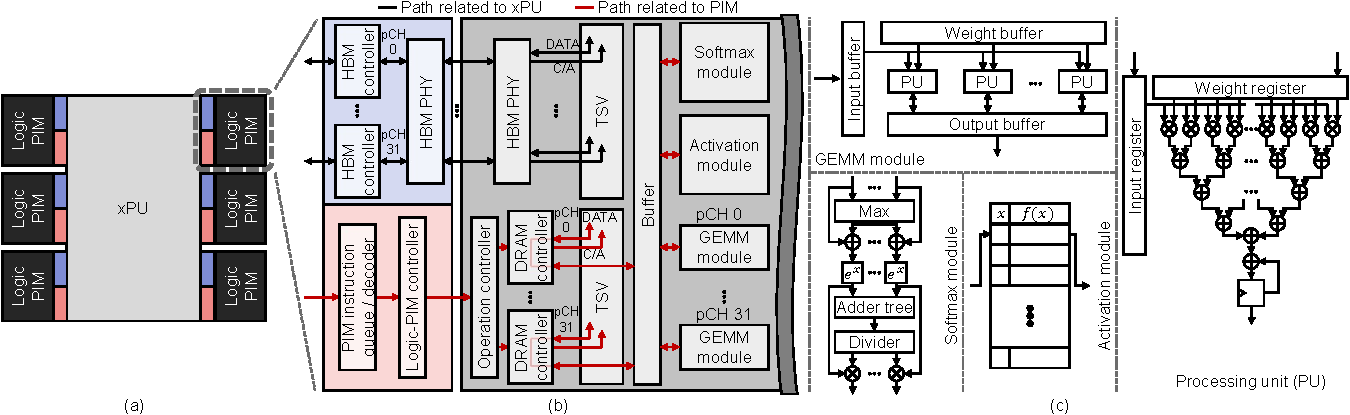
\includegraphics[width=0.95\textwidth]{figures/chip.pdf}
  \vspace{-0.08in}
  \caption{(a) Top view of Duplex chip, (b) the architecture of Logic-PIM, and (c) the details of processing units.
  }
  \label{fig:duplex_chipdesign}
  \vspace{-0.1in}
\end{figure*}


The MoE and attention layers, which exhibit low \opb ranging from 1 to 32, face challenges when performed using the PIM architectures in prior studies~\cite{isca-2021-hbm-pim, isscc-2022-aim, asplos-2024-attacc, asplos-2024-neupim}, which place processing units inside DRAM dies. 
The banks share external wires within a single pseudo channel, allowing them to read data from only one bank at a time. 
In contrast, a PIM architecture places an internal computing unit in each bank, where all those can read data from its bank simultaneously, improving effective memory bandwidth.
While such PIM architectures are effective for extremely low-\opb operations (under 1) by exploiting the high internal bandwidth of DRAM dies, their performance is suboptimal for operations in the MoE and attention (GQA) layers. 
Populating more processing units with these PIM architectures~\cite{isca-2021-hbm-pim, isscc-2022-aim} is not cost-effective due to the significant area overhead involved in integrating processing units with DRAM processing technologies.
In commercially available PIM devices such as~\cite{isca-2021-hbm-pim, isscc-2022-aim}, even when the compute-to-memory-bandwidth ratio is one, processing units already occupy 27\% and between 20\% and 25\% of the DRAM die area, respectively.

Considering the required range of \opb (1 to 32), we design the target architecture for low-\opb units to achieve 4$\times$ the memory bandwidth of conventional HBM, with a compute-to-memory-bandwidth ratio of eight. 
Because the logic die can leverage the logic process~\cite{imw-2017-hbm-dram-technology, todaes-2021-nmp-cnn-hbm}, more processing units can be placed on the logic die than on the DRAM die of the same area.
However, merely adding processing units to the logic die does not offer any memory bandwidth benefits compared to \highp.
We observe \emph{a reduction in the TSV pitch in recent HBMs from 50um to 22um}~\cite{SKhynix-tsv-pitch}, which allows quadrupling the number of TSVs with only a 9\% area overhead (detailed in Section~\ref{sec:eval:area_overhead}).
Motivated by this technology trend, we propose \lowp, which increases the internal bandwidth by adding more TSVs and adds processing units to the logic die which can utilize the logic process.



\subsection{Microarchitecture of \lowp}
In designing \lowp, we set two main objectives of minimizing modifications to DRAM and reducing the internal DRAM datapath length to reduce the energy required to read data~\cite{MICRO-2017-fine-grained-dram}.
In providing 4$\times$ higher memory bandwidth, simply increasing the bandwidth of each bank incurs a significant overhead of quadrupling the prefetch size of the banks and increasing the I/O datapath width by 4$\times$.
This results in a 77\% increase in the size of the DRAM banks and necessitates changes to the DRAM bank layout~\cite{MICRO-2017-fine-grained-dram}.

Instead, we increase the number of banks operating simultaneously without modifying the structure of the DRAM banks.
Conventional memory systems share bank I/O and bank group I/O, allowing data to be read from only one bank at a time. 
We place switches between each bank I/O and separate their paths to enable reading data simultaneously from multiple banks (see Fig.~\ref{fig:duplex_microarchitecture}).
Because reading data from the same bank group takes twice as long (tCCD\_L) as that from different bank groups (tCCD\_S), we simultaneously read from eight banks to achieve 4$\times$ higher bandwidth. 
We divide 16 banks for a single rank and a pseudo channel into upper (colored red in Fig.~\ref{fig:duplex_microarchitecture}) and lower banks and make each group of eight banks operate as one unit, which we refer to as bank bundle.


We integrate additional TSVs for \lowp in the conventional HBM's power TSV area instead of data TSV area. 
To transmit data read from each bank in a \bankbundle to the logic die, we must connect the \lowp-path I/O from each bank group to the TSVs.
Adding TSVs for \lowp to the existing data TSV area would result in longer datapaths from each bank group, thereby consuming more energy~\cite{MICRO-2017-fine-grained-dram}. 
By placing \lowp TSVs near the areas for power TSVs, we reduce the length of \lowp-path I/O from each bank to TSVs and minimize the wiring overhead.

\highp and \lowp can read data simultaneously using \bankbundle parallelism.
\lowp sends the same command/address (C/A) to the target \bankbundle, thus simultaneously reading data from eight banks. \lowp reads a total of 512 bits from two banks per bank group at intervals defined by tCCD\_L, which travels to the I/O buffer in the additional TSVs installed, and the data is transferred through the TSV to the logic die. 
In the case of the \highp path, a simple switch separates it from the \lowp datapath, allowing \highp to read data from the other bank bundles even when \lowp is accessing data.
Each pseudo channel comprises four bank bundles, organized into two ranks with two bank bundles per rank, with indices set from one to four. 
To prevent \bankbundle conflicts when simultaneously using \lowp and \highp, we strategically allocate the weights of models and KV matrices considering the index of bank bundles.


\begin{figure}[!tb]
  \center
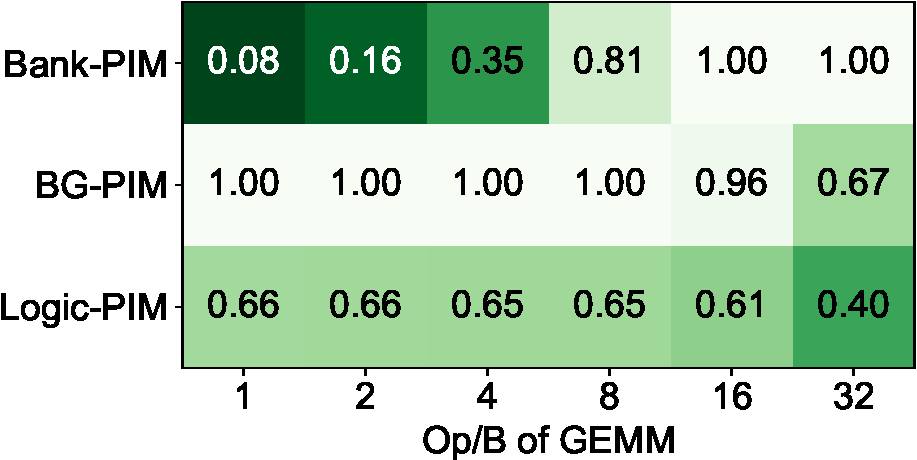
\includegraphics[width=0.64\columnwidth]{figures/edap.pdf}
  \vspace{-0.05in}
  \caption{The normalized energy-delay-area product (EDAP) of Bank-PIM, BankGroup-PIM, and Logic-PIM by \opb of FP16 GEMM operation. Weight matrix is (16384$\times$4096). Details about each architecture are in Section~\ref{sec:experimental_setup}.
  }
  \label{fig:edap}
  \vspace{-0.10in}
\end{figure}



\subsection{\duplex Architecture}

Fig.~\ref{fig:duplex_chipdesign}(a) shows the overall design of \duplex. 
An \highp in the center is responsible for high-\opb operations. 
A \lowp (Fig.~\ref{fig:duplex_chipdesign}(b)) is connected to a conventional HBM controller to read data for high-Op/B operations, and is also connected to a \lowp controller, which controls the processing units in \lowp. 
Unlike HBM controllers, the \lowp controller does not receive data from \lowp.
Instead, all computations are performed on the logic die. 
Thus, only control pins are used to connect \lowp with the controller, resulting in minimal pin overhead.

\lowp consists of a simple DRAM controller for fetching data from HBM, GEMM modules for performing low-\opb GEMM operations, a buffer, and modules for softmax and activation functions. 
The \lowp controller sends \lowp the starting addresses of weights and inputs, as well as the dimensions of the GEMM to the operation controller. Upon receiving a compute request from the \lowp controller, the operation controller fetches data via the DRAM controller and performs computations using the GEMM module.
The activation module handles the activation in the MoE layers, and the softmax module is used for the attention layer.


\subsection{Comparing \duplex with prior PIM architecture}
\duplex is more suited for contemporary LLMs than prior PIM architectures that add processing units to DRAM dies.
\duplex exhibits a better energy-delay-area product (EDAP) for GEMM operations above 8 \opb over prior DRAM die-based PIM architectures (see Fig.~\ref{fig:edap}, prior PIM architectures are detailed in Section~\ref{sec:experimental_setup}).
At \opb under eight, Bank-PIM, which can utilize the highest memory bandwidth, shows the best EDAP. 
However, as the \opb of operations increases, Bank-PIM, with its limited computing power, becomes less efficient compared to \lowp. 
Although BankGroup-PIM has the same memory bandwidth and computing power as \lowp, it always exhibits a higher (worse) EDAP due to having all its processing units and buffers on the DRAM die, resulting in a larger area overhead than \lowp.


\begin{figure}[!tb]
  \center
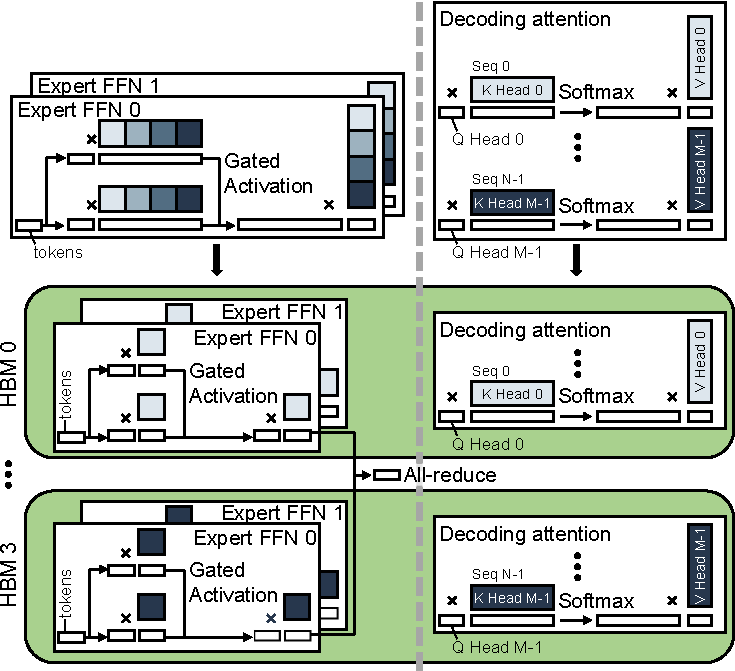
\includegraphics[width=0.85\columnwidth]{figures/job_distribution.pdf}
  \vspace{-0.1in}
  \caption{MoE and attention layers distributed among HBM stacks in a device. The shades of blue indicate which HBM each chunk of data is stored in.}
  \label{fig:duplex_job_distribution}
  \vspace{-0.1in}
\end{figure}
